%*********************************************************************
% RUCthesis: 中国人民大学本科生毕业论文模板
% Copyright 2020  Qiu Renxiang
% 2020/06/06 v1.0 beta
%
%本文编写的依据是中国人民大学教务处2017年修订的《本科生毕业论文(设计)指导手册》
%本文的给出例子是参加“创新杯”学术比赛时编写的,本文的模板也是在此基础之上进行改造。
%本文基本满足手册中对本科生论文的格式要求,并自动生成图表目录并编号,引用和目录也都具有超链接。
%如果你有任何建议和疑问请发送邮件至qrx_math@ruc.edu.cn,协助我做的更好。
% 重要提示:
%   1. 请确保使用 UTF-8 编码保存
%   2. 请使用 XeLaTeX编译
%   3. 修改、使用、发布本文档请务必遵循 LaTeX Project Public License
%   4. 不需要的注释可以尽情删除
%*********************************************************************
\documentclass[12pt,UTF8]{ctexart}
\usepackage{amsmath}
\usepackage{float}
\usepackage{cite}
\usepackage{listings}
\usepackage{graphicx}
\usepackage{epstopdf}
\usepackage{booktabs}
\usepackage{multirow}
\usepackage{geometry}
\usepackage{appendix}
\usepackage{hyperref}
\usepackage{enumerate}
\usepackage{threeparttable}
\usepackage{fancyhdr}
\usepackage{setspace}
\usepackage[T1]{fontenc}
\usepackage{mathptmx}%Times New Roman字体
\usepackage{titletoc}
\usepackage{fontspec}
\usepackage{pdfpages}
\usepackage{tikz}
\usepackage{etoolbox}
\usepackage{xcolor}
\usepackage{caption}
\usepackage{array}
\usepackage{amssymb}



%图表目录重定义
\renewcommand {\thetable} {\thesection{}.\arabic{table}}
\renewcommand {\thefigure} {\thesection{}.\arabic{figure}}

%\CTEXsetup[number={\chinese{section}}]{section}
%\CTEXsetup[name={(,)},number={\chinese{subsection}}]{subsection}
%\CTEXsetup[number={\arabic{subsubsection}}]{subsubsection}

%本科学生毕业论文要求纵向打印,页边距的要求为:
%上(T):2 cm
%下(B):2 cm
% 左(L):1.5 cm
% 右(R):1.5 cm
% 装订线(T):0.5 cm
% 装订线位置(T):左
\geometry{a4paper,left = 2cm,right = 1.5cm,top = 2cm,bottom= 2cm}


% 页眉:学校标志(教务处主页提供下载):
% 高度为0.98 cm,宽度为4.13 cm,居中放置。
% 页码采用10.5号宋体字,居中放置,格式为:第1页。
\pagestyle{fancy}
\lhead{}
\chead{
\includegraphics[width = 4.13cm,height = 0.98cm]{head.png}}
\rhead{}
\lfoot{}
\rfoot{}

%目录和引用超链接
\hypersetup{
colorlinks=true,
linkcolor=black,
citecolor=black
}

\begin{document}

\newcommand\dunderline[3][-1pt]{{%
  \setbox0=\hbox{#3}
  \ooalign{\copy0\cr\rule[\dimexpr#1-#2\relax]{\wd0}{#2}}}}


\begin{titlepage}
  \vspace*{6mm}
  \centering

  
\includegraphics[scale = 1.5]{title.jpg}

  \vspace*{-3mm}

  \zihao{1}\textbf{\heiti{本科生毕业论文(设计)}}

  \vspace{14mm}

  \zihao{1}\textbf{\heiti 我是大标题}

  \vspace{3mm}

  \begin{spacing}{1.2}
    \LARGE\selectfont{\textbf{\heiti ——我是小标题}}
  \end{spacing}

  \vspace{10mm}

  \flushleft
  \begin{spacing}{1.3}
    \hspace{27mm}\heiti\LARGE\selectfont{\textbf{论文编码:}\dunderline[-10pt]{1pt}{\makebox[78mm][c]{20020525}}}
  
    \hspace{27mm}\heiti\LARGE\selectfont{\textbf{学\hspace{14mm}院:}\dunderline[-10pt]{1pt}{\makebox[78mm][c]{信息学院}}}

    \hspace{27mm}\heiti\LARGE\selectfont{\textbf{专\hspace{14mm}业:}\dunderline[-10pt]{1pt}{\makebox[78mm][c]{数学与应用数学}}}

    \hspace{27mm}\heiti\LARGE\selectfont{\textbf{年\hspace{14mm}级:}\dunderline[-10pt]{1pt}{\makebox[78mm][c]{2018级}}}

    \hspace{27mm}\heiti\LARGE\selectfont{\textbf{学\hspace{14mm}号:}\dunderline[-10pt]{1pt}{\makebox[78mm][c]{2018202044}}}
    
    \hspace{27mm}\heiti\LARGE\selectfont{\textbf{学生姓名:}\dunderline[-10pt]{1pt}{\makebox[78mm][c]{邱任翔}}}

    \hspace{27mm}\heiti\LARGE\selectfont{\textbf{指导教师:}\dunderline[-10pt]{1pt}{\makebox[78mm][c]{林枫}}}
    
    \hspace{27mm}\heiti\LARGE\selectfont{\textbf{完成日期:}\dunderline[-10pt]{1pt}{\makebox[78mm][c]{2020.06.06}}}
  \end{spacing}

  \vspace{25mm}

\end{titlepage}


\newpage
\renewcommand{\abstractname}{\textbf{\Large \heiti 摘要}}
\renewenvironment{abstract}{%
    \par\small
    \noindent\mbox{}\hfill{\bfseries \abstractname}\hfill\mbox{}\par
    \vskip 2.5ex}{\par\vskip 2.5ex} 
%中文摘要及关键词放在扉页一、外文摘要及关键词放在扉二,页码编排为Ⅰ,Ⅱ,设置页眉
\begin{abstract}
%1.5倍行距
\begin{onehalfspace}
近年来互联网的广泛使用引发了信息的爆炸式增长,个性化推荐系统作为解决“信息过载”问题的有效工具应运而生,通过算法帮助用户过滤信息,减少了用户需要处理的信息量。目前,个性化推荐系统已经广泛应用于搜索引擎、电子商务、社交娱乐等网络平台,在人们日常使用的过程中随处可见。然而,个性化推荐系统的广泛应用也带来了“信息窄化”、用户信息泄露等问题,个性化推荐系统对于用户信息搜寻成本的具体影响变得更为复杂。

本文将用结构方程模型来分析信息搜寻成本的变化对个性化推荐系统的用户使用意愿的影响情况。

基于研究得出的结论,本文从现实中存在的个性化推荐精度不足、信息窄化以及个人信息的侵害等方面的问题出发,提出了对于未来个性化推荐优化的展望。在算法方面,通过使用深度学习与知识图谱等前沿技术与算法提高个性化推荐的精确程度。在个人信息使用与信息窄化的问题上,平台可以增加相应调节选项,提高用户的自主选择性。其次,也可以通过提高推荐过程的可解释性来增强用户对推荐系统的信任度与满意度。另外,还需要政府部门完善个人信息保护的法律法规、社会舆论与公共部门发挥监督与监管作用,以及企业上下游齐发力,共同降低个人隐私泄露的风险。
\\[12pt]
\textbf{\textbf{\heiti 关键词:}}个性化推荐;感知信息搜寻成本;结构方程模型;
\end{onehalfspace}
\end{abstract}
\setcounter{page}{1}
\pagenumbering{Roman}
\cfoot{\footnotesize \thepage}
\newpage

\newcommand{\enabstractname}{\textbf{\Large Abstract}}
\newenvironment{enabstract}{%
    \par\small
    \noindent\mbox{}\hfill{\bfseries \enabstractname}\hfill\mbox{}\par
    \vskip 2.5ex}{\par\vskip 2.5ex}  
\begin{enabstract}
\begin{doublespace}
English Abstract
\\[12pt]
\textbf{Keywords:}Personalized Recommendation;
\end{doublespace}
\end{enabstract}
\cfoot{\thepage}
\newpage
\cfoot{}
\renewcommand\contentsname{目\ 录}
\renewcommand\listfigurename{插\ 图}
\renewcommand\listtablename{表\ 格}
\tableofcontents
\listoffigures
\listoftables
\newpage
\setcounter{page}{1}
\setcounter{table}{0}
\setcounter{figure}{0}
\pagenumbering{arabic}
\pagestyle{fancy}
\cfoot{\footnotesize 第 \thepage 页}
% 按照自然段依次排列,每段起行空两格,回行顶格。12号宋体字,(重点文句,12号宋体字,加粗),1.25倍行距。
%正文、注释双面打印,编排页码,自第1页起,设置页眉。
\begin{spacing}{1.25}
\section{绪论}
\subsection{研究意义}
\subsubsection{理论意义}
\setcounter{table}{0}
\setcounter{figure}{0}
\section{文献综述}
\setcounter{table}{0}
\setcounter{figure}{0}
\section{问卷设计}
\subsection{测量指标的设计}
\subsection{样本选择}
\setcounter{table}{0}
\setcounter{figure}{0}
\section{数据分析与结果讨论}

\begin{table}[H]
\centering
\caption{样本的特征统计}
\label{tab:ybtj}
\begin{tabular}{@{}cllll@{}}
\toprule
\multicolumn{1}{l}{\textbf{样本统计特征}}          & \textbf{分类} & \textbf{频次} & \textbf{有效百分比} & \textbf{累计百分比} \\ \midrule
\multirow{2}{*}{性别}                          & 男           & 100         & 29.3\%         & 29.3\%         \\
                                             & 女           & 241         & 70.7\%         & 100.0\%        \\ \midrule
\multirow{3}{*}{学历}                          & 专科及以下       & 29          & 8.5\%          & 8.5\%          \\
                                             & 本科          & 297         & 87.1\%         & 95.6\%         \\
                                             & 硕士及以上       & 15          & 4.4\%          & 100.0\%        \\ \midrule
\multicolumn{1}{l}{\multirow{2}{*}{常用的推荐算法}} & 基于内容        & 193         & 56.6\%         & 56.6\%         \\
\multicolumn{1}{l}{}                         & 基于协同过滤      & 148         & 43.4\%         & 100.0\%        \\ \bottomrule
\end{tabular}
\end{table}


\begin{table}[H]
\centering
\caption{用户常用个性化平台数据特征}
\label{tab:gxhpt}
\begin{tabular}{@{}lll@{}}
\toprule
\multicolumn{1}{c}{\textbf{个性化推荐平台}} & \multicolumn{1}{c}{\textbf{频次}} & \multicolumn{1}{c}{\textbf{有效百分比}} \\ \midrule
购物平台类(淘宝、京东、拼多多等)                    & 304                             & 89.1\%                             \\
视频娱乐类(b站、爱奇艺等)                      & 244                             & 71.6\%                             \\
社交分享类(小红书、抖音、微博等)                    & 207                             & 60.7\%                             \\
知识问答类(知乎、quora等)                     & 203                             & 59.5\%                             \\
生活美食类(美团、饿了吗等)                       & 187                             & 54.8\%                             \\
旅游出行类(携程旅行,大众点评等)                    & 82                              & 24.0\%                             \\ \bottomrule
\end{tabular}
\end{table}
。
\begin{table}[H]
\centering
\caption{各测量指标的统计分析(N = 5,min = 1,max = 5)}
\label{tab:clzb}
\begin{tabular}{@{}llllllllll@{}}
\toprule
\textbf{因素}                                                               & \textbf{测量指标}& \textbf{均值} & \textbf{标准偏差} & \textbf{方差} & \textbf{偏度} & \textbf{峰度} \\ \midrule
\multirow{3}{*}{\begin{tabular}[c]{@{}l@{}}时间成本降低\\  \textbf{(3.64)}\end{tabular}} & TC1                       & 3.92        & 0.806         & 0.65        & -0.601      & 0.471       \\
                                                                          & TC2                      & 3.6         & 0.923         & 0.852       & -0.458      & 0.026       \\
                                                                          & TC3                      & 3.4         & 1.005         & 1.01        & -0.228      & -0.431      \\ \midrule
\multirow{3}{*}{\begin{tabular}[c]{@{}l@{}}心理成本增加\\  \textbf{(3.37)}\end{tabular}} & PC1                      & 3.48        & 1.1           & 1.209       & 0.519       & -0.37       \\
                                                                          & PC2                       & 3.17        & 1.07          & 1.146       & 0.28        & -0.556      \\
                                                                          & PC3                       & 3.47        & 0.981         & 0.962       & 0.262       & -0.416      \\ \midrule
\multirow{3}{*}{\begin{tabular}[c]{@{}l@{}}金钱成本降低\\  \textbf{(3.99)}\end{tabular}} & MC1                      & 4.02        & 0.945         & 0.894       & -0.782      & 0.212       \\
                                                                          & MC2                       & 3.94        & 0.899         & 0.808       & -0.69       & 0.394       \\
                                                                          & MC3                       & 4.01        & 0.874         & 0.765       & -0.66       & 0.183       \\ \midrule
\multirow{4}{*}{\begin{tabular}[c]{@{}l@{}}风险成本增加\\  \textbf{(3.45)}\end{tabular}} & RC1                      & 3.43        & 0.91          & 0.829       & -0.285      & -0.055      \\
                                                                          & RC2                       & 3.1         & 0.959         & 0.919       & 0.202       & -0.274      \\
                                                                          & RC3                       & 3.65        & 0.969         & 0.939       & -0.373      & -0.407      \\
                                                                          & RC4                       & 3.62        & 1             & 1           & -0.293      & -0.532      \\ \midrule
\multirow{3}{*}{\begin{tabular}[c]{@{}l@{}}使用意愿\\  \textbf{(3.56)}\end{tabular}}   & UW1                       & 3.51        & 0.916         & 0.839       & -0.285      & -0.184      \\
                                                                          & UW2                       & 3.54        & 0.862         & 0.743       & -0.566      & 0.627       \\
                                                                          & UW3                       & 3.64        & 0.889         & 0.79        & -0.541      & 0.466       \\ \bottomrule
\end{tabular}
\end{table}
\subsection{信度及效度检验}
\subsubsection{信度检验}
信度(reliability)是指根据测量指标所测得结果的一致性或稳定性, 反映被测特征真实程度的指标。按照所测信度的范围不同,又分为内在信度和外在信度。
\begin{enumerate}[(1)]
    \item 内在信度:是指对一组问题是否测量同一概念,常用Cronbach's $\alpha$值、因子载荷和CR值三个指标进行检测。本文中检验问卷中设计的各测量指标是否可以一致地测量该因素。
    \item 外在信度:是指不同时间对相同的测试者测得的结果是否一致。一般而言, 不同测试的结果越一致,则结果的误差越小,外在信度就越高。
\end{enumerate}

由于研究条件限制,本文仅对内在信度进行检验。各指标需要满足:Cronbach's $\alpha$在0.70以上则表示内在信度较好(参考值见表\ref{tab:cronbach});因子载荷需要大于0.5,而CR值(construct reliability)表示组合信度,其值在0.60以上则说明模型的内在质量理想,公式为:
\begin{equation}
    CR=\frac{\left (  \sum \lambda _{i}\right )^{2}}{\left [\left (  \sum \lambda _{i}\right )^{2}+\sum \theta   \right ]}
\end{equation}
其中,$\lambda _{i}$为指标变量在潜在变量上的标准化因子载荷值,$\theta$是标准化残差,i=1,2,3。
\begin{table}[H]
\centering
\caption{Cronbach's $\alpha$ 系数信度表}
\label{tab:cronbach}
\begin{tabular}{@{}cc@{}}
\toprule
\textbf{Cronbach's $\alpha$ 值}              & \textbf{可信度} \\ \midrule
Cronbach's $\alpha$ \textless 0.3           & 不可信          \\
0.3 $\leq$ Cronbach's $\alpha$ \textless 0.4 & 勉强可信         \\
0.4 $\leq$ Cronbach's $\alpha$ \textless 0.5 & 尚且可信         \\
0.5 $\leq$ Cronbach's $\alpha$ \textless 0.7 & 一般可信         \\
0.7 $\leq$ Cronbach's $\alpha$ \textless 0.9 & 比较可信         \\
Cronbach's $\alpha$ $\geq$ 0.9               & 非常可信         \\ \bottomrule
\end{tabular}
\end{table}

模型中各因素的内在信度检验如表\ref{tab:rel}所示,从表中可见,各因素的测量指标Cronbach`s $\alpha$均在0.70以上;测量指标的标准化因子载荷值都基本大于0.5,基本适配指标理想;CR值均在0.6以上,表明测量的内部一致性很好。因此本研究所选取的测量指标具有较高的信度。
\begin{table}[H]
\centering
\caption{信度检验}
\label{tab:rel}
\begin{tabular}{@{}ccccccc@{}}
\toprule
\textbf{因素} & \textbf{测量指标} & \textbf{\begin{tabular}[c]{@{}c@{}}标准化因子载荷\\ $\lambda$\end{tabular}} & \textbf{\begin{tabular}[c]{@{}c@{}}信度系数\\ $\lambda^{2}$\end{tabular}} & \textbf{\begin{tabular}[c]{@{}c@{}}误差变异量\\ $1-\lambda^{2}$\end{tabular}} & \textbf{CR}            & \textbf{Cronbach`s $\alpha$} \\ \midrule
时间成本降低      & TC1           & 0.743                                                                & 0.552                                                                 & 0.448                                                                    &                        &                              \\
Time Cost          & TC2           & 0.71                                                                 & 0.504                                                                 & 0.496                                                                    & 0.714                  & 0.701                        \\
            & TC3           & 0.563                                                                & 0.317                                                                 & 0.683                                                                    &                        &                              \\ \midrule
心理成本增加      & PC1           & 0.674                                                                & 0.454                                                                 & 0.546                                                                    &                        &                              \\
Psychological Cost          & PC2           & 0.648                                                                & 0.42                                                                  & 0.58                                                                     & 0.629                  & 0.698                        \\
            & PC3           & 0.474                                                                & 0.225                                                                 & 0.775                                                                    &                        &                              \\ \midrule
金钱成本降低      & MC1           & 0.59                                                                 & 0.348                                                                 & 0.652                                                                    &                        &                              \\
Money Cost          & MC2           & 0.67                                                                 & 0.449                                                                 & 0.551                                                                    & 0.704                  & 0.700                        \\
            & MC3           & 0.731                                                                & 0.534                                                                 & 0.466                                                                    &                        &                              \\ \midrule
风险成本增加      & RC1           & 0.522                                                                & 0.272                                                                 & 0.728                                                                    & \multirow{4}{*}{0.729} & \multirow{4}{*}{0.722}       \\
Risk Cost          & RC2           & 0.591                                                                & 0.349                                                                 & 0.651                                                                    &                        &                              \\
            & RC3           & 0.752                                                                & 0.566                                                                 & 0.434                                                                    &                        &                              \\
            & RC4           & 0.664                                                                & 0.441                                                                 & 0.559                                                                    &                        &                              \\ \midrule
使用意愿        & UW1           & 0.826                                                                & 0.682                                                                 & 0.318                                                                    &                        &                              \\
Users' Willingness          & UW2           & 0.845                                                                & 0.714                                                                 & 0.286                                                                    & 0.872                  & 0.872                        \\
            & UW3           & 0.828                                                                & 0.686                                                                 & 0.314                                                                    &                        &                              \\ \bottomrule
\end{tabular}
\end{table}
\subsubsection{效度检验}
效度(validity) 是指衡量测量指标所测得结果是否能真实反映被测特征的程度的统计指标。效度通常又分为聚合效度和区分效度两种。聚合效度(convergent validity)要求同属一个因素的测量指标之间有高度的相关性;区分效度(discriminate validity)是要求不同因素所对应的测量指标之间的相关性小。一般采用平均方差抽取量(Average Variance Extracted,AVE值)通过因子载荷量计算的表示聚合效度的指标值。计算公式如下:
\begin{equation}
    AVE=\frac{\left (  \sum \lambda _{i}^{2}\right )}{\left [\left (  \sum \lambda _{i}^{2}\right )+\sum \theta   \right ]}
\end{equation}

\begin{table}[H]
\centering
\caption{效度检验}
\label{tab:val}
\begin{tabular}{@{}lllllll@{}}
\toprule
\textbf{} & \textbf{RC} & \textbf{MC} & \textbf{PC} & \textbf{TC} & \textbf{UW} & \textbf{AVE} \\ \midrule
RC        & 0.637       &             &             &             &             & 0.407        \\
MC        & 0.364       & 0.666       &             &             &             & 0.444        \\
PC        & -0.295      & -0.181      & 0.604       &             &             & 0.366        \\
TC        & 0.028       & 0.447       & -0.246      & 0.676       &             & 0.458        \\
UW        & -0.047      & 0.446       & -0.273      & 0.779       & 0.833       & 0.694        \\ \bottomrule
\end{tabular}
\end{table}
验。
\subsection{模型检验}
\subsubsection{结构方程模型}
由于测量指标已经通过信度和效度检验,因此进一步对理论模型进行检验,检验结果如图\ref{fig:sem}所示
\begin{figure}[H]
\centering
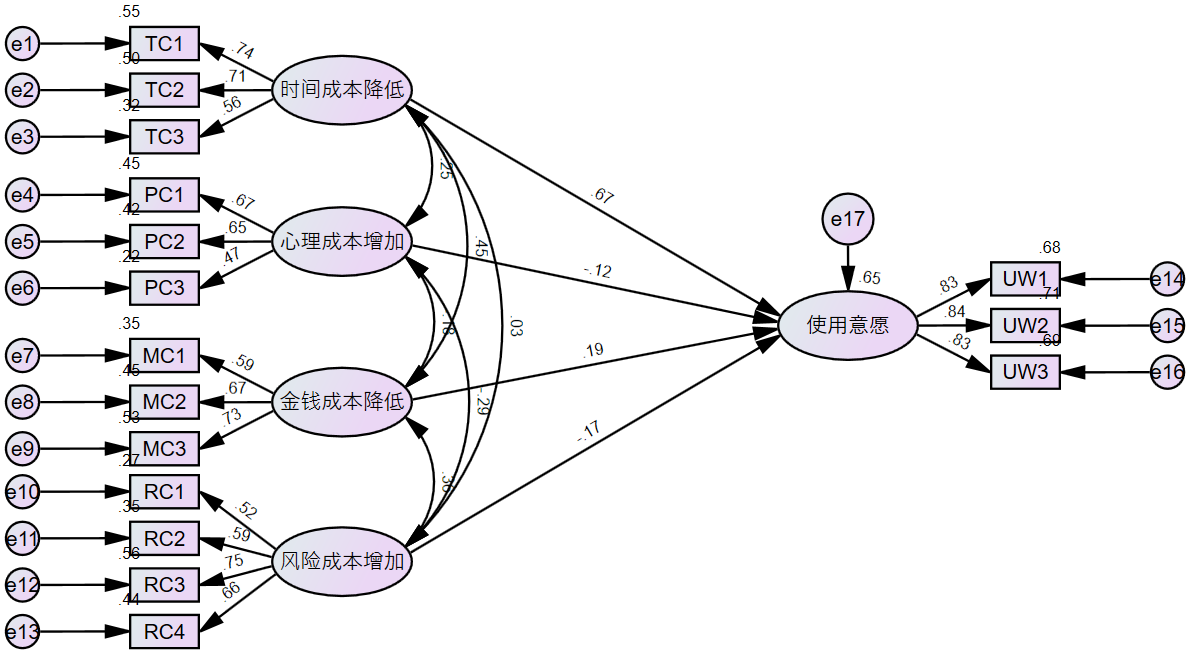
\includegraphics[scale = .6]{sem.png}
\caption{标准化结构方程模型}
\label{fig:sem}
\end{figure}

\begin{table}[H]
\centering
\caption{结构方程拟合指标}
\label{tab:sem}
\begin{tabular}{@{}lllll@{}}
\toprule
\textbf{指标种类}    & \textbf{指标名称}         & \textbf{评价标准}   & \textbf{本模型拟合值} & \textbf{模型适配判断} \\ \midrule
\textbf{绝对拟合度指标} & $\chi^{2}$            &                 & 262.554         &                 \\
\textbf{}        & df                    &                 & 94              &                 \\
\textbf{}        & 近似误差均方根(RMSEA)        & \textless{}0.08 & 0.073           & 是               \\
\textbf{}        & 残差均方根(RMR)            & \textless{}0.05 & 0.066           & 否               \\
\textbf{}        & 标准残差均方根(SRMR)            & \textless{}0.05 & 0.046           & 是               \\
\textbf{}        & 拟合优度(GFI)             & $\geq$0.9       & 0.915           & 是               \\
                 & 调整拟合优度(AGFI)          & $\geq$0.9       & 0.901           & 是               \\ \midrule
\textbf{增值拟合度指标} & 常规拟合度(NFI)            & $\geq$0.9       & 0.855           & 否               \\
\textbf{}        & 相对拟合指数(RFI)           & $\geq$0.9       & 0.815           & 否               \\
\textbf{}        & 增量拟合指数(IFI)           & $\geq$0.9       & 0.902           & 是               \\
\textbf{}        & 非常规拟合度(TLI)           & $\geq$0.9       & 0.873           & 否               \\
\textbf{}        & 比较拟合指数(CFI)           & $\geq$0.9       & 0.901           & 是               \\ \midrule
\textbf{简约拟合度指标} & 卡方自由度比($\chi^{2}/df$) & \textless{}3    & 2.793           & 是               \\
\textbf{}        & PGFI                  & $\geq$0.5       & 0.632           & 是               \\
\textbf{}        & PNFI                  & $\geq$0.5       & 0.670           & 是               \\
\textbf{}        & PCFI                  & $\geq$0.5       & 0.705           & 是               \\
\textbf{}        & CN值                   & $\geq$340       & 341             & 是               \\ \bottomrule
\end{tabular}
\end{table}
。
\begin{table}[H]
\centering
\caption{路径检验和标准化路径系数}
\label{tab:road}
\begin{threeparttable}
\begin{tabular}{@{}llllll@{}}
\toprule
\textbf{路径}              & \textbf{Estimate} & \textbf{标准误差} & \textbf{t值} & \textbf{P值} & \textbf{标准化路径系数} \\ \midrule
使用意愿\textless{}---时间成本降低 & 0.772             & 0.102         & 7.597       & ***         & 0.67             \\
使用意愿\textless{}---心理成本增加 & -0.205            & 0.095         & -2.157      & 0.023       & -0.124           \\
使用意愿\textless{}---金钱成本降低 & 0.252             & 0.107         & 2.358       & 0.018       & 0.186            \\
使用意愿\textless{}---风险成本增加 & -0.228            & 0.092         & -2.483      & 0.013       & -0.171           \\ \bottomrule
\end{tabular}
\begin{tablenotes}
    \item 注:***表示p<0.001。
\end{tablenotes}
\end{threeparttable}
\end{table}
以显著性水平为0.05,结合上表数值即可判断本研究提出对的研究假设成立与否,结果如表\ref{tab:result}所示:
\begin{table}[H]
\centering
\caption{变量假设关系的检验结果}
\label{tab:result}
\begin{tabular}{@{}lll@{}}
\toprule
\textbf{假设编号} & \textbf{研究假设}            & \textbf{检验结果} \\ \midrule
H1            & 时间成本降低对用户的个性化推荐使用意愿有正向影响 & 显著            \\
H2            & 心理成本增加对用户的个性化推荐使用意愿有负向影响 & 显著            \\
H3            & 金钱成本降低对用户的个性化推荐使用意愿有正向影响 & 显著            \\
H4            & 风险成本增加对用户的个性化推荐使用意愿有负向影响 & 显著            \\ \bottomrule
\end{tabular}
\end{table}

\subsubsection{不同偏好推荐算法组}
首先,我们对不同偏好推荐算法组,采用多群组结构方程模型进行比较分析,模型结果如图\ref{fig:nr}和图\ref{fig:xt}所示。
\begin{figure}[H]
\centering
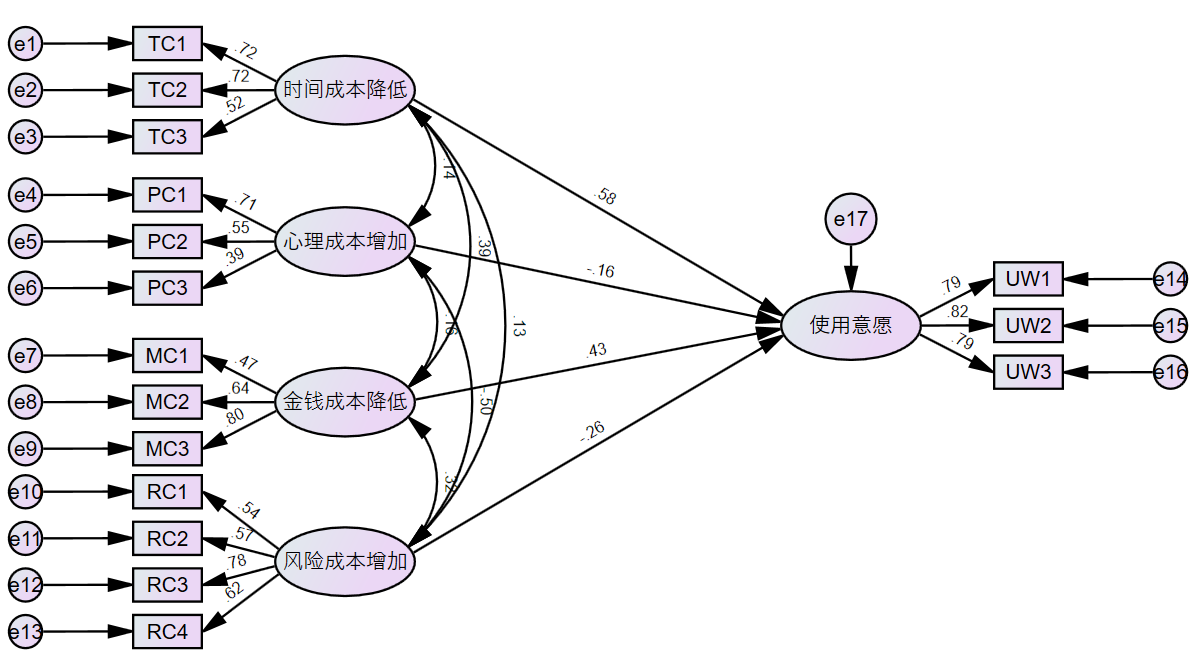
\includegraphics[scale = .5]{nr.png}
\caption{基于内容的个性化推荐算法组(N=193)}
\label{fig:nr}
\end{figure}
\begin{figure}[H]
\centering
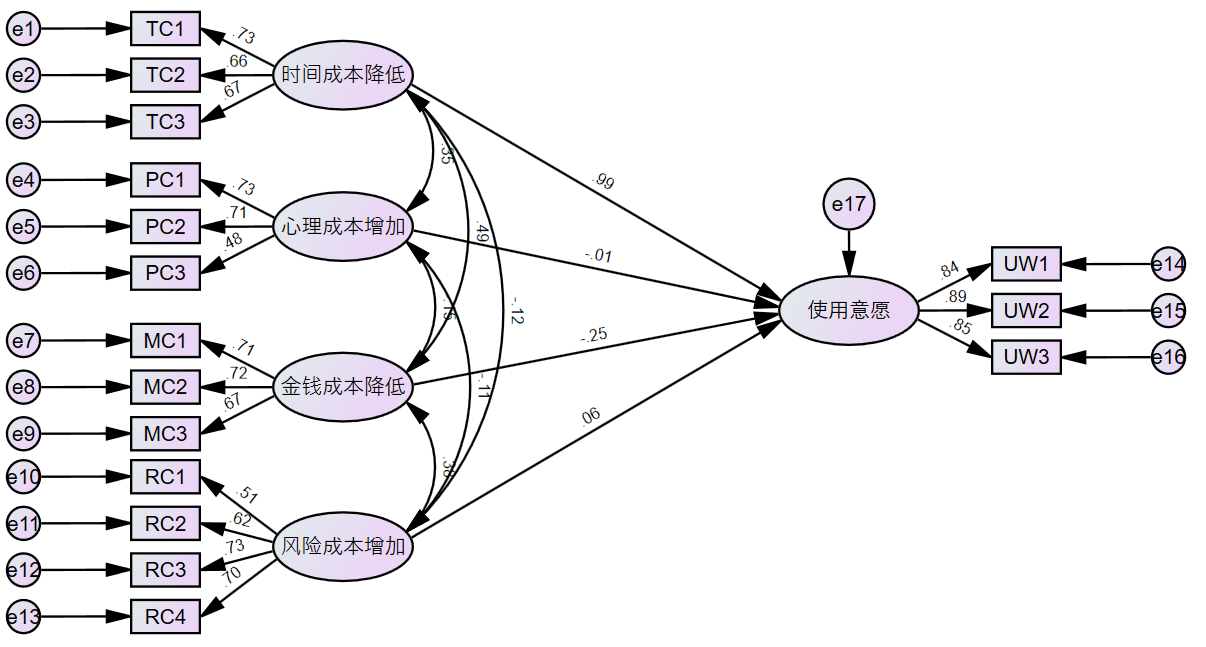
\includegraphics[scale = .5]{xt.png}
\caption{基于协同过滤的个性化推荐算法组(N=148)}
\label{fig:xt}
\end{figure}
\begin{table}[H]
\centering
\caption{不同常用算法组限制性与非限制性的拟合指标}
\label{tab:constrain1}
\begin{tabular}{@{}ccc@{}}
\toprule
\textbf{统计检验量} & \textbf{非限制性} & \textbf{限制性} \\ \midrule
$\chi^{2}$     & 385.342       & 414.078      \\
df             & 188           & 203          \\
$\chi^{2}$变化量  &               & 28.736       \\
df变化量          &               & 15           \\
显著性            &               & 0.017        \\ \bottomrule
\end{tabular}
\end{table}
由表\ref{tab:constrain1}可以看出:限制性模型和非限制性模型的卡方差值为28.736,自由度差为15,对应的P值为0.01<0.05,达到显著。说明这两组模型是有显著差异的,也就是说基于内容和基于协同过滤组在这四条路径之间是存在差异的,进一步对每一个路径进行差异分析:
\begin{table}[H]
\centering
\caption{基于内容和基于协同过滤组的路径系数差异性分析}
\label{tab:pair}
\begin{threeparttable}
\begin{tabular}{@{}ccccccc@{}}
\toprule
\textbf{}                & \multicolumn{2}{c}{\textbf{\begin{tabular}[c]{@{}c@{}}基于内容的算法\\ (N=193)\end{tabular}}} & \multicolumn{2}{c}{\textbf{\begin{tabular}[c]{@{}c@{}}基于协同过滤的算法\\ (N=148)\end{tabular}}} & \multicolumn{2}{c}{\textbf{\begin{tabular}[c]{@{}c@{}}Pairwise Parameter \\ Comparisons\end{tabular}}} \\ \midrule
                         & 标准化估计                                      & P值                                        & 标准化估计                                       & P值                                         & T值                                                 & P值                                                \\
使用意愿\textless{}---时间成本降低 & 0.578                                      & ***                                       & 0.989                                       & ***                                        & 2.582                                              & 0.005                                             \\
使用意愿\textless{}---心理成本增加 & -0.16                                      & 0.134                                     & -0.006                                      & 0.955                                      & 1.161                                              & 0.123                                             \\
使用意愿\textless{}---金钱成本降低 & 0.431                                      & ***                                       & -0.255                                      & 0.05                                       & -4.040                                             & 0.000                                             \\
使用意愿\textless{}---风险成本增加 & -0.256                                     & 0.014                                     & 0.059                                       & 0.611                                      & 2.013                                              & 0.022                                             \\ \bottomrule
\end{tabular}
\begin{tablenotes}
    \item 注:***表示p<0.001。
\end{tablenotes}
\end{threeparttable}
\end{table}


\subsubsection{不同性别组和不同平台类别组}
由于不同平台组如果两两相互比较需要比较15次,表格中只给出购物平台类和知识问答类组的对比情况。
\begin{table}[H]
\centering
\caption{不同性别组限制性与非限制性的拟合指标}
\label{tab:constrain2}
\begin{tabular}{@{}cccll@{}}
\toprule
\multicolumn{1}{l}{} & \multicolumn{2}{l}{\textbf{不同性别组}} & \multicolumn{2}{l}{\textbf{不同平台组(购物平台类和知识问答类)}} \\ \midrule
\textbf{统计检验量}       & \textbf{非限制性}    & \textbf{限制性}    & \textbf{非限制性}    & \textbf{限制性}    \\ \midrule
$\chi^{2}$           & 401.505          & 411.537         & 1247.383         & 1256.511        \\
df                   & 188              & 203             & 619              & 639             \\
$\chi^{2}$变化量        &                  & 10.032          &                  & 9.128           \\
df变化量                &                  & 15              &                  & 20              \\
显著性                  &                  & 0.817           &                  & 0.981           \\ \bottomrule
\end{tabular}
\end{table}
由表\ref{tab:constrain2}可以看出:不同性别组限制性模型和非限制性模型的卡方差值为10.032,自由度差为15,对应的P值为0.817>0.05,并不显著。购物平台类和知识问答类两种平台组中知识问答类限制性模型和非限制性模型的卡方差值为9.128,自由度差为20,对应的P值为0.981>0.05,也并不显著。对于其余14组不同平台组的对比,P值也皆大于0.05,表面不显著。说明这两个变量的两组模型并没有显著差异的,即不同性别和不同平台并不显著干扰该模型。但出于研究考虑我们将路径系数的估计结果整理如下表\ref{tab:multi}:
 
\begin{table}[H]
\centering
\caption{多群组分析结果(标准化路径系数值)}
\label{tab:multi}
\begin{threeparttable}
\begin{tabular}{@{}llllll@{}}
\toprule
\textbf{路径} & \textbf{}         & \textbf{H1} & \textbf{H2} & \textbf{H3} & \textbf{H4} \\ \midrule
性别          & 男                 & 0.696***    & -0.249**    & 0.132       & -0.027      \\
            & 女                 & 0.633***    & -0.075      & 0.229*      & -0.223*     \\ \midrule
平台类别        & 购物平台类(淘宝、京东、拼多多等) & 0.742***    & -0.053      & 0.111       & -0.104      \\
            & 知识问答类(知乎、quora等)  & 0.593***    & -0.173*     & 0.122       & -0.146      \\
            & 社交分享类(小红书、抖音、微博等) & 0.58***     & -0.231**    & 0.191       & -0.163      \\
            & 生活美食类(美团、饿了吗等)    & 0.753***    & -0.19**     & 0.052       & -0.073      \\
            & 旅游出行类(携程旅行,大众点评等) & 0.637**     & -0.102      & 0.067       & -0.014      \\
            & 视频娱乐类(b站、爱奇艺等)    & 0.636***    & -0.153**    & 0.159       & -0.234*     \\ \bottomrule
\end{tabular}
\begin{tablenotes}
    \item 注:*表示p<0.05,**表示p<0.01,***表示p<0.001。
\end{tablenotes}
\end{threeparttable}
\end{table}


\setcounter{table}{0}
\setcounter{figure}{0}
\section{总结和展望}
\subsection{研究结论}

本文通过对假设的模型进行验证,主要得出的结论有:
\begin{enumerate}[(1)]
    \item 时间成本降低
    \item 相比于全部样本
    \item 时间成本降低
    \item 对于较常使用
\end{enumerate}

\subsection{研究的不足}
由于客观条件限制,本次研究在以下三个方面仍存在不足:
\begin{enumerate}[(1)]
    \item 在实证调查中
    \item 本次问卷调查的对象主要为大学生群体,且本科生、985重点大学生居多,调查样本有一定局限性。
    \item 最终统
\end{enumerate}

\subsection{对现状的反思}
\newpage
\end{spacing}
\nocite{*}
\bibliographystyle{abbrv}
\addcontentsline{toc}{section}{\heiti 参考文献}
\bibliography{references.bib}
\appendix
\end{document}